\chapter{Background}
\label{chap2}

This chapter provides the general framing of the phenomena I investigated throughout this thesis, alongside the tools utilized to either replicate these phenomena within detailed simulations or compensate for their negative effects on the accuracy of the captured data and subsequent algorithmic decision-making. 

\section{Machine Learning (ML)}

 Machine learning is a class of algorithms designed to construct systems that automatically improve through experience. These systems are capable of autonomously learning the underlying relationships between input data and target output, relieving developers from the need to understand these relationships themselves and, eventually, manually modeling complex rules or hard-coding solutions \cite{ml-trends-persp, useful-things-ml}. 

 Early practical applications of machine learning included probabilistic text classification, unsupervised clustering \cite{MacQueen1967SomeMF},  automated decision making \cite{decision-trees} and text recognition \cite{handwritten, lenet}. Over time, the tasks assigned to ML models grew increasingly complex, becoming the dominant methodology for computer vision applications, speech recognition, natural language processing, and more. 

The primary working principle behind the functionality of most supervised ML models is the approximation of a function that, based on its inputs, calculates an output. In parallel, a loss metric is defined, quantifying the error between the model's approximated function's result and the desired output \cite{ml-trends-persp}. Through iterative training, the model gets exposed to multiple examples of input-output pairs, making the approximated function more and more complex and robust to new inputs.

The ability of ML models to autonomously uncover complex relationships and translate them into complex mathematical expressions, without requiring the developer to explicitly define them, was the primary reason why machine learning was elected as the exclusive tool for mapping the measured GRVI values to their ground truth counterparts. Surely, much like many other physical phenomena, the identified sources of error could be modeled and, eventually, a mathematical function could be constructed, handling the calculation of the true GRVI values. By employing machine learning, though, I drastically accelerated this process and yet achieved impressive results.

\subsection{ML Inference on Accelerators and Edge Devices}

Despite the aforementioned advantages of ML, it has its own caveats. One of its most important downsides is that most of the modern widely used model architectures are associated with a high computational cost. During training, many ML algorithms require repeated optimizations over large datasets and high-dimensional parameter matrices, making the training process increasingly demanding as the size and complexity of the model increases \cite{large-scale-ml}. To compensate for the large volume of matrix operations that naturally exceed the practical capabilities of conventional CPUs, researchers have shifted towards parallel platforms for the training of large models.

Computational constrains, however are not limited to the training stage. Once trained, a model must still execute its primary task, with that being providing predictions based on input data. Large models, such as deep neural networks, may contain millions of parameters, requiring large numbers of floating-point operations and memory accesses, leading to increased inference latency, memory usage, and energy consumption \cite{efficient-DNN}. Similar limitations appear in classical ML algorithms, specifically ensemble methods, where increasing the number and complexity of decision trees increases the amount of model information that must be stored and processed. The overhead of these models becomes particularly important when ML models are transferred from powerful workstations to edge devices, where available memory, computational resources, and energy are severely restricted \cite{splitting-stump}. Consequently, reducing the model's size and computational requirements is necessary to enable efficient inference on resource-constrained devices.

Since the final products of this thesis are machine learning models designed for inference in embedded devices, it was important to consider the limitations of these platforms. Therefore, for the design of the final model architectures, compromises had to be made in terms of their complexity, while still achieving promising predictive performance.

\section{Vegetation Indices}

In the context of remote sensing, it has been discovered that analyzing a field's spectral response generally provides the majority of the information needed regarding its vegetation's vigor. That said, relying solely on the raw spectral bands reflected by the field could be unreliable, since these measurements are also influenced by surrounding factors, such as the soil's color, shadows, moisture levels and more. In order to establish a more robust solution for quantifying the intensity of phenomena observed during the monitoring of plants, researchers have developed several mathematical combinations of the distinct spectral bands, known as vegetation indices (VIs) \cite{review-veg-index}. 

The major advantage of using vegetation indices is the ability to monitor complex phenomena occurring during the life cycle of crops, without the need to investigate every contributing variable, while also being isolated from several instances of lingering environmental noise throughout the process. VIs describe aspects of the observed vegetation’s development, such as its growth stage, health status, physiological and environmental conditions, and, in the case of crops, the amount of attention needed per part of the field and the validation of crop uniformity across it by simply quantifying the presence of factors related to these aspects, without the need for further interpretation \cite{vi-in-precision-agr}.


\subsection{Green-Red Vegetation Index (GRVI)}

Green-Red Vegetation Index (GRVI) in particular is a normalized spectral index defined as:
\[
GRVI = \frac{\rho_g - \rho_r}{\rho_g + \rho_r}
\]
where $\rho_g$ and $\rho_r$ are the reflectances of the visible green and red bands, respectively. The most common applications where GRVI is used include plant phenology monitoring.

Compared to other commonly used vegetation indices, such as NDVI, EVI, and GNDVI, GRVI offers several practical and application-specific advantages. Since it relies solely on visible spectral bands, GRVI can be accurately calculated using low-cost visible-band sensors, including properly calibrated RGB cameras \cite{gpp-grvi-phenology}. Beyond being highly cost-effective compared to methods that require expensive equipment, GRVI's reliance on visible radiation also ties it directly to the studied directional lighting phenomena. Visible shifts in the radiation reflected by the crops' canopy actually cause measurable changes to the metric.

Another significant advantage of GRVI relative to other vegetation indices is its sensitivity to visible changes in the vegetation's color. Because of this attribute, GRVI has proven to be effective for monitoring plant greenness across different stages of their lifespan \cite{gpp-grvi-phenology, rs-grvi-phenology}, despite its reliance on less complex systems for its calculation. Considering that part of the development of the digital twin was assigning plants different versions of the same material, creating unevenness in the inherent red-green ratio of the meshes across the simulated field, a metric that would be able to depict this unevenness was needed.

Lastly, another reason for selecting GRVI as the core metric in this work was its susceptibility to atmospheric noise. Especially in ground-based systems, as the one simulated, GRVI values are inconsistent, depending on sun position, cast shadows, viewing geometry, etc. \cite{impact_of_sunlight_conditions}. As discussed later, these factors affected the examined metric during the simulation too. Manipulating them produced a large volume of synthetic data, used as examples of how non-ideal monitoring conditions can harm the extracted information and how, with the use of ML, they can be corrected to approach their true values.

\section{Bidirectional Reflectance Distribution Function (BRDF)} \label{brdf}

The Bidirectional Reflectance Distribution Function (BRDF) describes how incident light arriving from one direction to a surface is reflected towards different directions above this surface. It can also be described as the ratio of the radiance dL($\theta_r$, $\phi_r$) reflected by the surface in the direction ($\theta_r$, $\phi_r$) to the incident irradiance dE($\theta_i$, $\phi_i$) that arrives at the surface due to the source from the direction ($\theta_i$, $\phi_i$). Mathematically:
\[
BRDF = f_r(\theta_i, \phi_i; \theta_r, \phi_r) = \frac{dL_r(\theta_r, \phi_r)}{ dE_i(\theta_i, \phi_i)},
\]
where $\theta_i$ is the incident zenith angle, $\theta_r$ is the reflected zenith angle, $\phi_i$ is the incident azimuth angle and $\phi_r$ is the reflected azimuth angle.

If the reflected radiation changes when the reflected direction ($\theta_r$, $\phi_r$) changes, then the reflector is characterized as anisotropic. The canopy of a crop field behaves as an anisotropic reflector, thus causing the studied phenomenon where different parts of the field appear more illuminated than others. This dependence on the reflected direction is described by the canopy's BRDF.

\begin{figure} [htb]
    \centering
    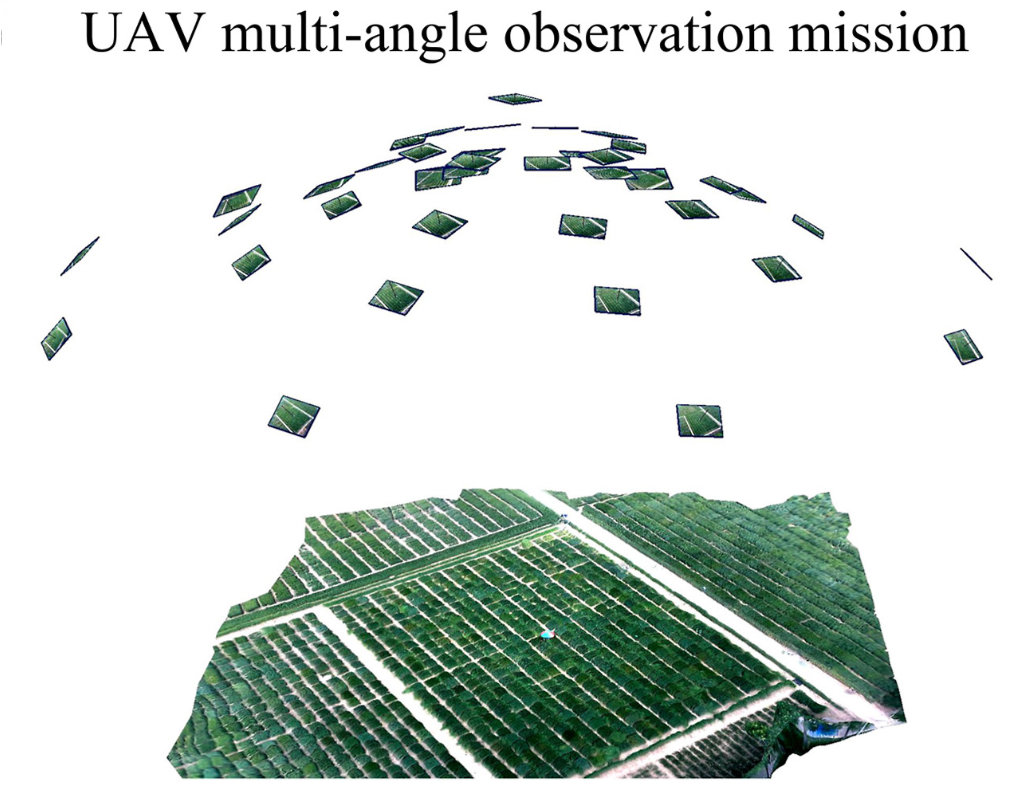
\includegraphics[width=1\linewidth]{images/uav-multiangle.png}
    \caption{BRDF anisotropy examined from various viewing angles with the help of unmanned aerial vehicles (UAV) \cite{uav-bdrf}}
    \label{drones}
\end{figure}

Figure ~\ref{drones} shows a multi-angle UAV observation geometry, proposed by Mi et al. \cite{uav-bdrf} for studying the BRDF anisotropy phenomenon, as it appears on a wheat field's canopy. It can be seen that, depending on the sun-canopy-sensor geometry, several parts of the canopy appear more occluded than others, despite the lack of interference between the light source and the field's canopy.

Multiple instances of this dependence on the illumination source's direction appear in the synthetic dataset, both visually and, most importantly, radiometrically. Depending on the solar zenith angle, a difference as high as 384.79\% could be observed on the average perceived green- and red- band reflectance of the textures appearing in the area of interest, including the errors introduced by the calculation method.

\begin{figure}[htb]
    \centering
    
    \begin{subfigure}{0.48\linewidth}
        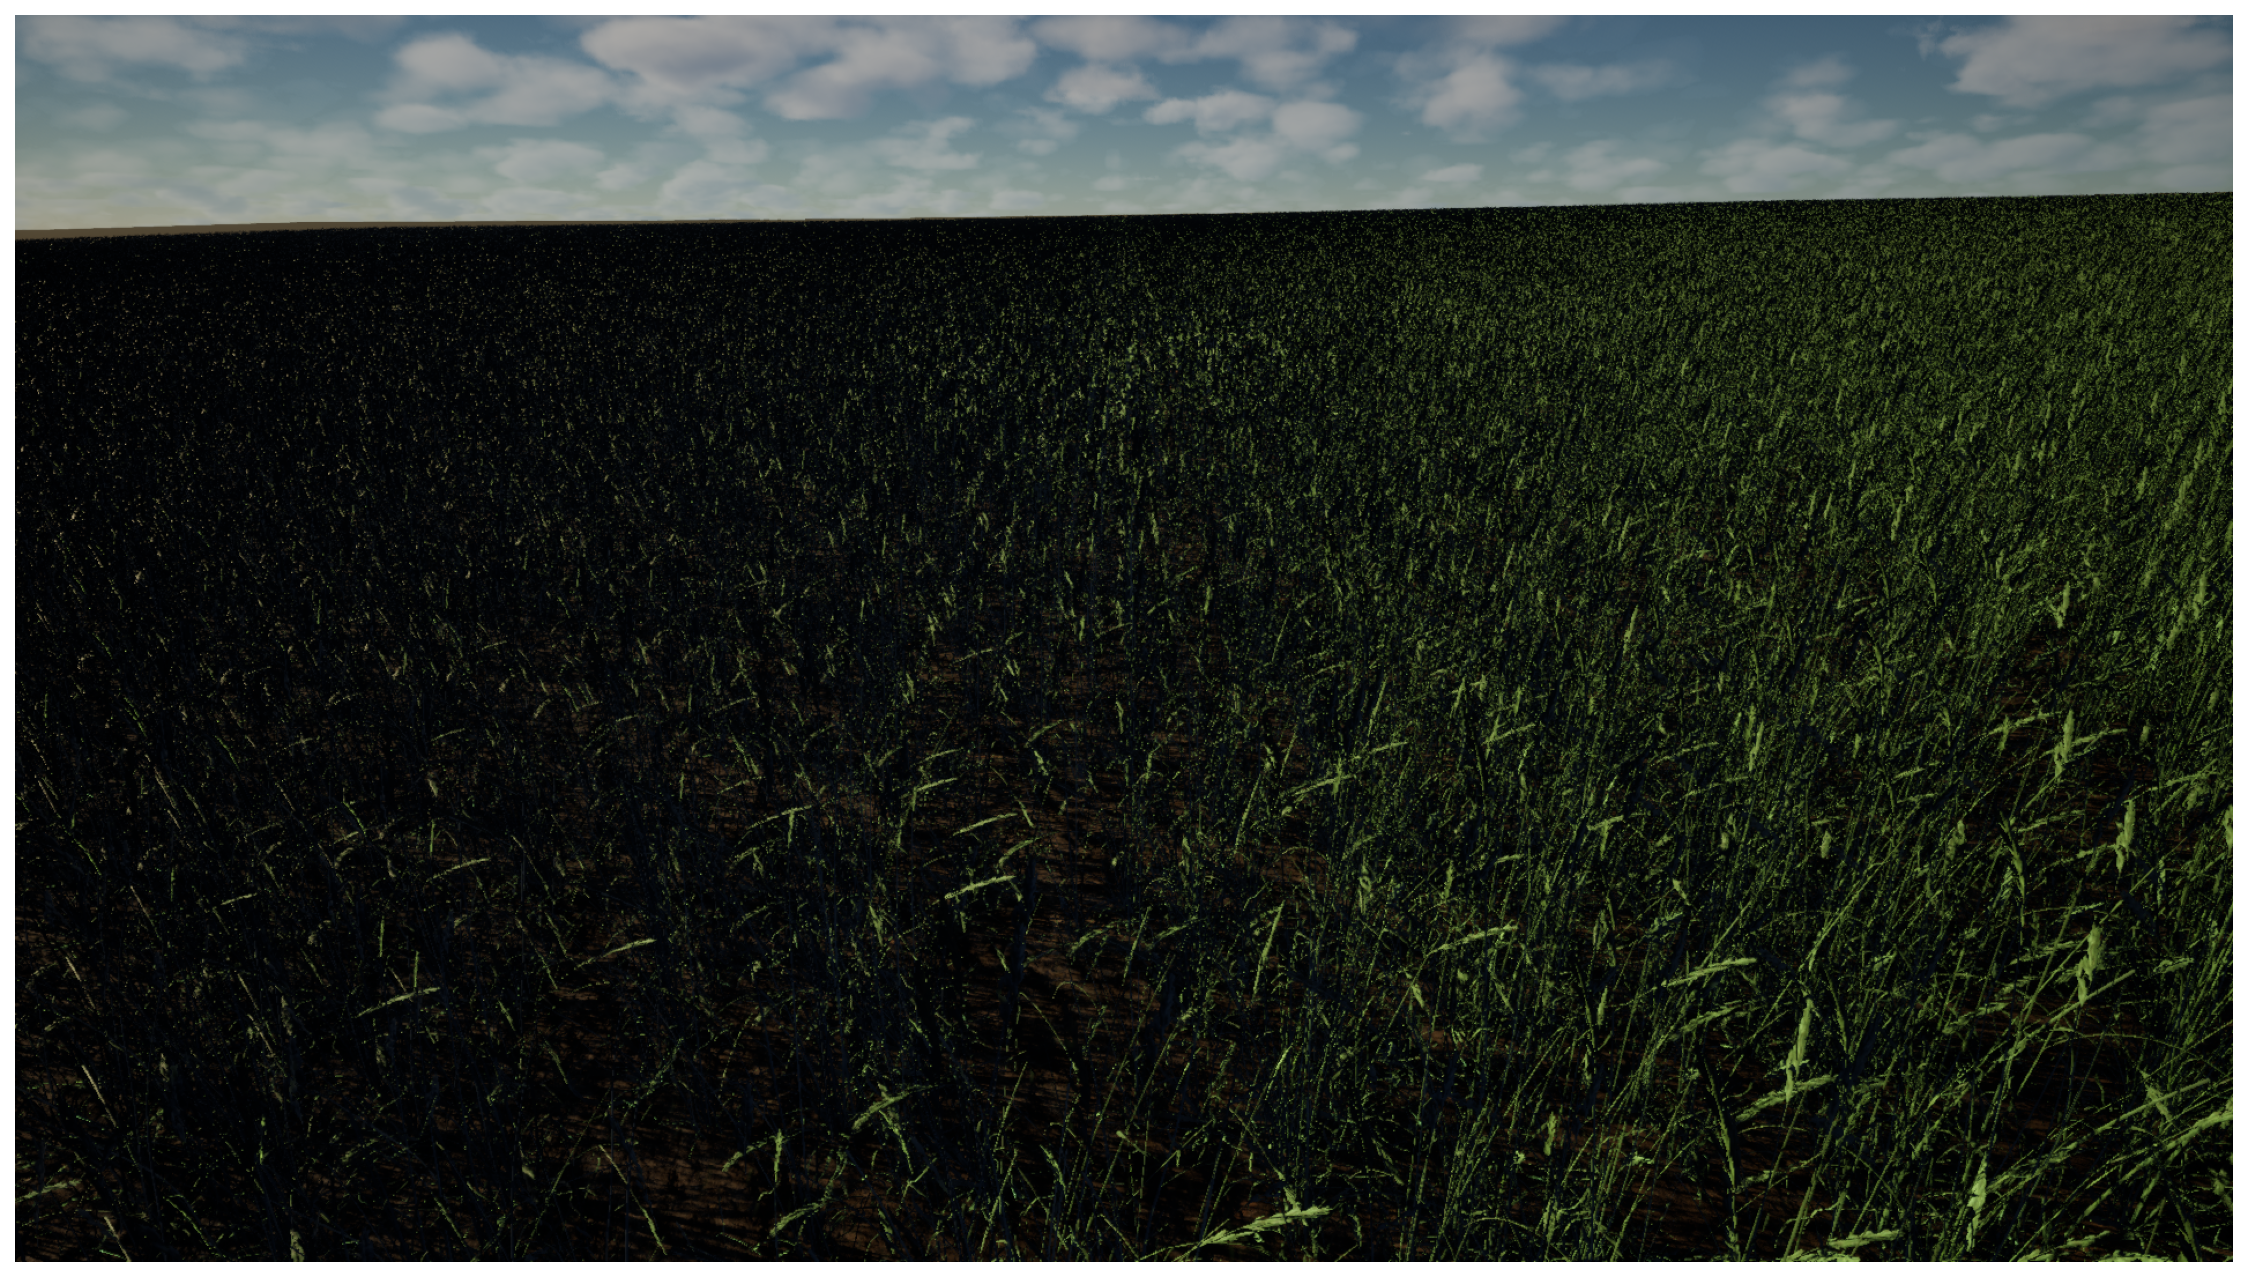
\includegraphics[width=\linewidth]{images/left.png}
        \caption{Image captured with SZA set to $104^o$}
        \label{leftgreen}
    \end{subfigure}\hfill
    \begin{subfigure}{0.48\linewidth}
        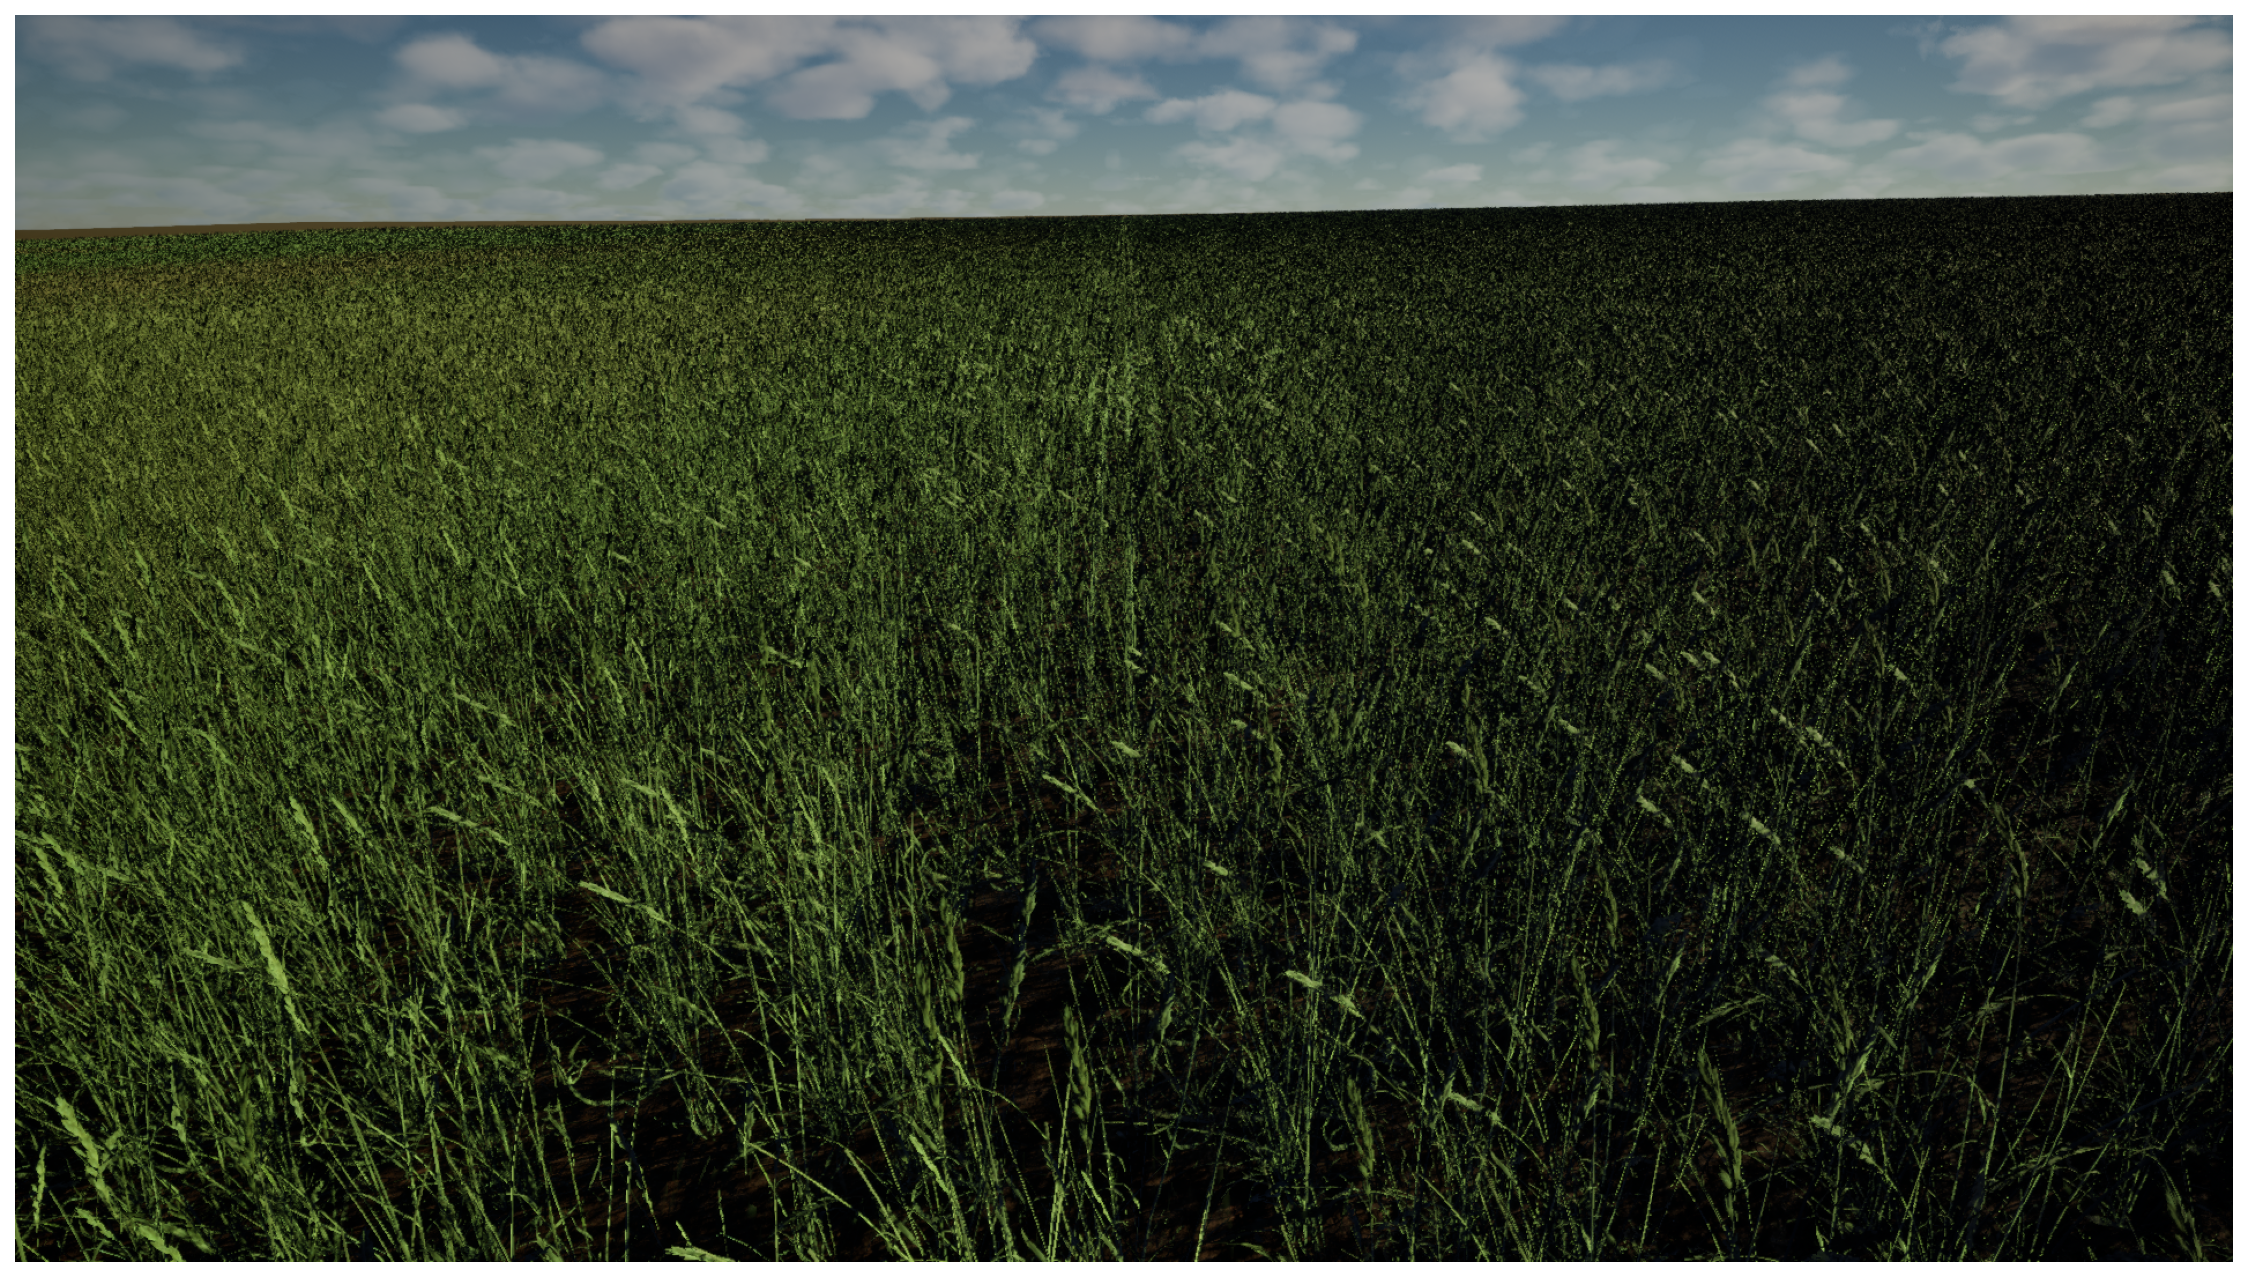
\includegraphics[width=\linewidth]{images/right.png}
        \caption{Image captured with SZA set to $-104^o$}
        \label{rightgreen}
    \end{subfigure}
    
        \caption{Images captured within the digital twin featuring the same scene under solar zenith angles (SZA) with opposite signs. In the left image (Figure~\ref{leftgreen}), the left part of the field appears more occluded than the right, despite the fact that illuminance is proven to be the same across it. The exact opposite is observed in the right image (Figure~\ref{rightgreen}).}
    \label{leftright}
\end{figure}




\section{Tools}
\subsection{Unreal Engine}

Unreal Engine (UE) is a 3D computer graphics game engine developed by Epic Games, capable of generating real-time 3D environments and interactive simulations \cite{wiki:unreal_engine}. In the past few years it has been explored as a digital twin design tool, as it offers a robust set of features, provided either natively or by external plugins, allowing the generation of ground truth data for model training and CV tasks. Apart from its capabilities, UE hosts a large community of developers who use it for digital twin design. This results in a plethora of third-party documentation, plugins, and sensors, all of which sped up the process of environment development and data extraction.

For the purpose of this work, Unreal Engine proved to offer sufficient tools for the implementation of a photorealistic digital environment, the simulation of natural phenomena fairly close to their real-life counterparts and tools capable of both validating these claims and storing the information needed to be gathered for the development of a robust machine learning model. Specifically, UE provides a large library of digital assets, such as foliage meshes and materials, a considerable amount of which are 3D scans of real flora and terrain materials \cite{quixel_megascans}, achieving an impressive level of detail. These assets, accompanied by the engine's built-in tools for procedural, yet not too artificial-looking, mesh placement and terrain manipulation, set an already promising foundation for the development of the environment. In parallel, the engine accurately simulated the various illumination conditions and the resulting light-surface interactions needed for the conducted experiments. Finally, UE supports the automated recording of all of the actors' parameters, especially while a programmed sequence of events occurs, enabling the synthesis of a machine learning dataset. 

\subsection{PyTorch}
PyTorch is an open-source Python library dedicated to the design, training, and inference of machine learning models. It is currently recognized as a standard for deep learning applications, as it combines both an intuitive API and high performance in terms of execution speed, attributed to both its optimized source code and its support for parallel computing platforms like CUDA \cite{torch-intro}. A small extent of PyTorch's capabilities was explored within the bounds of this work for the development of one of the proposed model architectures. 

\subsection{Scikit-learn}
Scikit-learn is an open-source machine learning Python library, widely established as a standard for classical ML, non-neural network algorithms \cite{scikit}. It provides multiple classical ML algorithms, data preprocessing and dimensionality reduction tools, and model evaluation and selection metrics. Scikit-learn was the primary library used for data preprocessing, while several of the algorithm implementations were used in an attempt to identify models that combine computational efficiency and satisfactory results in terms of predictive performance.

\subsection{cuML}
cuML is the scikit-learn counterpart for CUDA-enabled machines. It provides a plethora of classical machine learning algorithms optimized for training and inference on the supported graphical processing units (GPUs) while mimicking scikit-learn's interface \cite{nvidia_cuml_docs}. Apart from the algorithmic implementations of methods that can be found in scikit-learn, such as linear regression, clustering and ensemble algorithms, cuML also provides support for model architectures beyond these bounds. Specifically, the Forest Inference Library (FIL), which is part of cuML, is responsible for optimizing ensemble methods such as XGBoost, LightGBM, and non-inherently supported scikit-learn models for GPU inference \cite{nvidia_fil_2025}. 

cuML was the primary tool used for accelerating non-neural network models, leveraging its GPU-optimized implementations of tree-based ensemble methods. Since the inputs followed the formatting of tabular data, a dataset format where tree-based ensemble methods tend to excel, utilizing this framework ensured high performance both in prediction accuracy and computational speed. 

\subsection{TensorRT}

TensorRT is NVIDIA's SDK for high-performance deep learning inference on CUDA-enabled embedded platforms, such as the NVIDIA Jetson series. By providing a pre-trained neural network in ONNX format to TensorRT, it optimizes the graph by fusing adjacent layers to condense mathematical operations, and applies Post Training Quantization (PTQ), constraining the weights to lower-precision formats (INT8, FLOAT16, etc.) specified by the developer. Finally, it benchmarks multiple kernel implementations per layer and batch size, identifying the best-performing configuration, before compiling the optimized model. The output of this compilation is a file containing the quantized model weights, along with the execution graphs tailored specifically to the platform on which the compilation was performed. The complete compilation pipeline is illustrated in Figure~\ref{trt}, provided by the survey of Jeong et al. \cite{tensor-rt}.

\begin{figure} [htb]
    \centering
    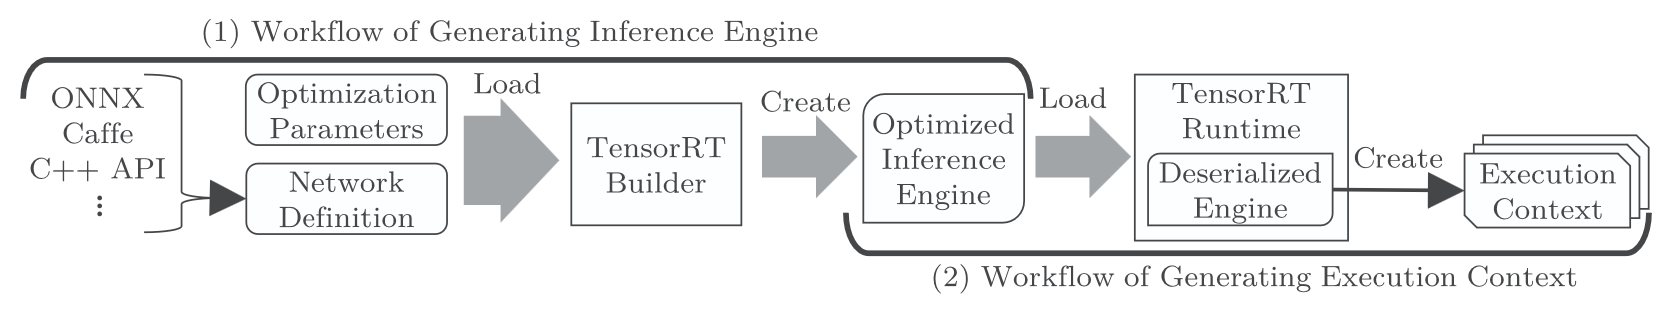
\includegraphics[width=1\linewidth]{images/Screenshot from 2026-09-16 22-44-53.png}
    \caption{Complete optimized model compilation using the TensorRT SDK} \cite{tensor-rt}
    \label{trt}
\end{figure}

Another capability of TensorRT is the profiling of the compiled model, providing performance insights for each individual layer of the compiled neural network.

Although deployment on a Jetson board was not feasible during the course of this research, primarily due to time constraints, experimentation with the TensorRT framework was still conducted. Specifically, the trained neural network models were compiled for execution on an NVIDIA RTX 2060 (6GB VRAM), to evaluate the accuracy loss caused by PTQ.